% Rapport revisite a partir des 20 entrainements archives, 9 octobre 2026.
% Regenerer : python paper/build_paper.py (figures et compilation XeLaTeX).
\documentclass[10pt,a4paper]{article}
\usepackage[a4paper,top=18mm,bottom=18mm,left=20mm,right=20mm,headheight=17pt]{geometry}
\usepackage{fontspec}
\setmainfont{Linux Libertine O}
\setsansfont{Inter}
\usepackage{amsmath,amssymb,unicode-math}
\setmathfont{STIX Math}
\usepackage{polyglossia}
\setdefaultlanguage{french}
\setotherlanguage{english}
\usepackage{microtype}
\usepackage{graphicx,booktabs,xcolor,array}
\usepackage{caption}
\usepackage{titlesec}
\usepackage{fancyhdr}
\usepackage[hidelinks]{hyperref}
\usepackage{float}
\usepackage{enumitem}
\usepackage{ragged2e}
\usepackage{tikz}
\usetikzlibrary{arrows.meta}
\usepackage{setspace}
\usepackage{needspace}
\setstretch{1.08}
\definecolor{navy}{HTML}{173951}
\definecolor{muted}{HTML}{526271}
\definecolor{rulegray}{HTML}{DCE3E7}
\definecolor{panelbg}{HTML}{F3F7F8}
\definecolor{accent}{HTML}{207C78}
\hypersetup{pdftitle={Biais d'estimation des critics : DDPG, TD3 et LayerNorm sur LunarLander},pdfauthor={Hachem Marzouk}}
\titleformat{\section}{\large\sffamily\bfseries\color{navy}}{\thesection.}{.48em}{}
\titlespacing*{\section}{0pt}{10pt plus 1pt}{3pt plus 1pt}
\titleformat{\subsection}{\normalsize\sffamily\bfseries\color{navy}}{}{0pt}{}
\titlespacing*{\subsection}{0pt}{6pt}{2pt}
\captionsetup{font=small,labelfont={bf,color=navy},skip=4pt,justification=justified}
\setlength{\parindent}{1em}
\setlength{\parskip}{2.2pt}
\setlength{\emergencystretch}{1.2em}
\setlength{\textfloatsep}{8pt}
\setlength{\intextsep}{7pt}
\setlength{\tabcolsep}{6pt}
\pagestyle{fancy}
\fancyhf{}
\fancyhead[L]{\footnotesize\sffamily\color{muted} MS2A · Reinforcement Learning}
\fancyhead[R]{\footnotesize\sffamily\color{muted} Étude expérimentale · 2026}
\renewcommand{\headrulewidth}{.3pt}
\renewcommand{\headrule}{\hbox to\headwidth{\color{rulegray}\leaders\hrule height \headrulewidth\hfill}}
\fancyfoot[L]{\footnotesize\sffamily\color{muted} Hachem Marzouk}
\fancyfoot[R]{\footnotesize\sffamily\color{muted}\thepage\,/\,4}
\renewcommand{\footrulewidth}{0pt}
\newcommand{\E}{\mathbb{E}}
\newcommand{\Q}{Q^{\pi}}
\newcommand{\mc}{G_t}
\newcommand{\smallnote}[1]{\par\vspace{2pt}{\small\color{muted}#1}\par}
\begin{document}
\thispagestyle{empty}
\vspace*{-9mm}
{\sffamily\footnotesize\bfseries\color{accent} REINFORCEMENT LEARNING \quad / \quad ÉTUDE EXPÉRIMENTALE}\par
\vspace{5pt}
\noindent{\sffamily\fontsize{18}{26}\selectfont\bfseries\color{navy}%
Biais d'estimation des critics\\[1pt]
DDPG, TD3 et Layer Normalization sur LunarLander}\par
\vspace{5pt}
{\sffamily\small Hachem Marzouk \quad\textcolor{rulegray}{|}\quad Master MS2A — Sorbonne Université \quad\textcolor{rulegray}{|}\quad Octobre 2026}\par
\vspace{7pt}
\noindent{\color{accent}\rule{\linewidth}{1.15pt}}\par
\vspace{5pt}
\noindent\textbf{Résumé.} Nous étudions le biais des critics de DDPG et TD3, avec et sans Layer Normalization (LN), sur \emph{LunarLander-v3} continu. Les prédictions sont comparées aux retours Monte-Carlo des politiques pendant 20 entraînements principaux (cinq par configuration, 300\,000 interactions), complétés par dix entraînements d'ablation sur DDPG. En fin d'apprentissage, DDPG surestime de $+133$ points contre $-20$ pour TD3. Avec LN, le biais de DDPG atteint $+1\,499$, alors que TD3+LN conserve un biais faible ($-12$). L'effet de LN dépend fortement de l'algorithme ; une ablation montre que, dans DDPG, la LN placée dans le seul critic ou le seul actor accroît déjà ce biais ($+837$ et $+352$).\par
\vspace{4pt}
\section{Problématique : biais du critic et choix de l’actor}
Dans DDPG, le \emph{critic} $Q_\theta(s,a)$ estime le retour futur si l'on choisit l'action $a$ dans l'état $s$, puis que l'on suit la politique $\pi_\phi$ de l'\emph{actor}. L'actor est précisément entraîné à augmenter $Q_\theta(s,\pi_\phi(s))$. Une erreur du critic n'est donc pas anodine : elle influence les actions qui seront apprises. La maximisation favorise les actions dont la valeur est accidentellement surestimée \cite{fujimoto2018,vanhasselt2010}.

Nous étudions deux questions : \textbf{(i)} TD3 donne-t-il une estimation des valeurs plus proche des retours observés que DDPG ? \textbf{(ii)} comment la LN, appliquée à l'actor et au(x) critic(s), modifie-t-elle cette estimation et la performance finale ? Un biais signé positif indique une surestimation, négatif une sous-estimation.

\section{DDPG et TD3 : cibles de Bellman et mises à jour}
Pour une politique déterministe $\pi$ et un facteur d'actualisation $\gamma$, la valeur véritable vérifie l'équation de Bellman :
\begin{equation}
\Q(s,a)=\E\!\left[\sum_{k\geq0}\gamma^k r_{t+k}\ \middle|\ S_t=s,A_t=a\right]
=\E\!\left[r_t+\gamma\Q(S_{t+1},\pi(S_{t+1}))\mid s,a\right].
\label{eq:bellman}
\end{equation}
DDPG approxime cette valeur par un réseau $Q_\theta$ entraîné en régression vers une \emph{cible de Bellman}. Pour une transition $(s,a,r,s',d)$, et en notant les copies lentes par une barre :
\begin{align}
\text{DDPG :}\quad y &= r+\gamma(1-d)\,Q_{\bar\theta}(s',\pi_{\bar\phi}(s')),\label{eq:ddpg}\\[-3pt]
\text{TD3 :}\quad y &= r+\gamma(1-d)\,\min_{i=1,2}Q_{\bar\theta_i}(s',\widetilde a'),
\quad \widetilde a'=\operatorname{clip}_{[-1,1]^2}\!\left(\pi_{\bar\phi}(s')+\operatorname{clip}_{[-c,c]^2}(\varepsilon)\right).\label{eq:td3}
\end{align}
Le critic principal minimise $\E[(Q_\theta(s,a)-y)^2]$ ; l'actor ajuste ses paramètres pour augmenter $\E[Q_{\theta_1}(s,\pi_\phi(s))]$. TD3 ajoute un second critic, du bruit gaussien borné $\varepsilon$ sur l'action cible et une mise à jour moins fréquente de l'actor \cite{lillicrap2016,fujimoto2018}. Son minimum rend la \emph{cible d'apprentissage} plus prudente, mais ne garantit ni une estimation exacte ni un biais toujours négatif.

\section{Protocole : évaluer le biais par Monte-Carlo}
L'environnement est \emph{LunarLander-v3} de Gymnasium, avec deux actions continues \cite{towers2024}. Nous comparons \textbf{DDPG, DDPG+LN, TD3 et TD3+LN} avec cinq graines par configuration (20 entraînements principaux, plus dix pour l'ablation DDPG). Chaque entraînement dure 300\,000 interactions ; les réseaux ont deux couches cachées de 256 neurones, $\gamma=0{,}99$, et des copies mises à jour lentement ($\tau=0{,}005$). La LN, lorsqu'elle est activée, est placée après les couches linéaires cachées, dans l'actor et le(s) critic(s). Le détail des hyperparamètres et le code figurent dans le dépôt associé.

Tous les 25\,000 pas, nous figeons l'actor, puis évaluons sa politique déterministe sur 20 épisodes. Pour chaque état-action visité, nous calculons le retour observé $G_t=\sum_{k\geq 0}\gamma^k r_{t+k}$ et l'erreur $Q_{\theta_1}(s_t,a_t)-G_t$. Le retour $G_t$ est un \emph{échantillon aléatoire}, non la véritable espérance $\Q(s_t,a_t)$. En moyennant ces écarts par épisode puis par graine, on estime le biais du critic sur les états visités par sa propre politique.

\smallnote{\textbf{Horizon.} Le retour de performance s'arrête à 1\,000 pas ; pour mesurer le biais, les épisodes encore actifs à ce seuil sont prolongés de 500 pas. Au fil des checkpoints, 29\,\% des épisodes d'évaluation de TD3 sans LN sont encore actifs à 1\,000 pas. Si $|r_t|\le R_{\max}$, l'erreur résiduelle est au plus $\gamma^{500}R_{\max}/(1-\gamma)$, soit $0{,}66\,\%$ de l'échelle $R_{\max}/(1-\gamma)$. Une troncature temporelle n'annule pas le bootstrap \cite{pardo2018}.}

\clearpage
\section{Résultats : biais estimé et retour obtenu}
\begin{figure}[H]
\centering
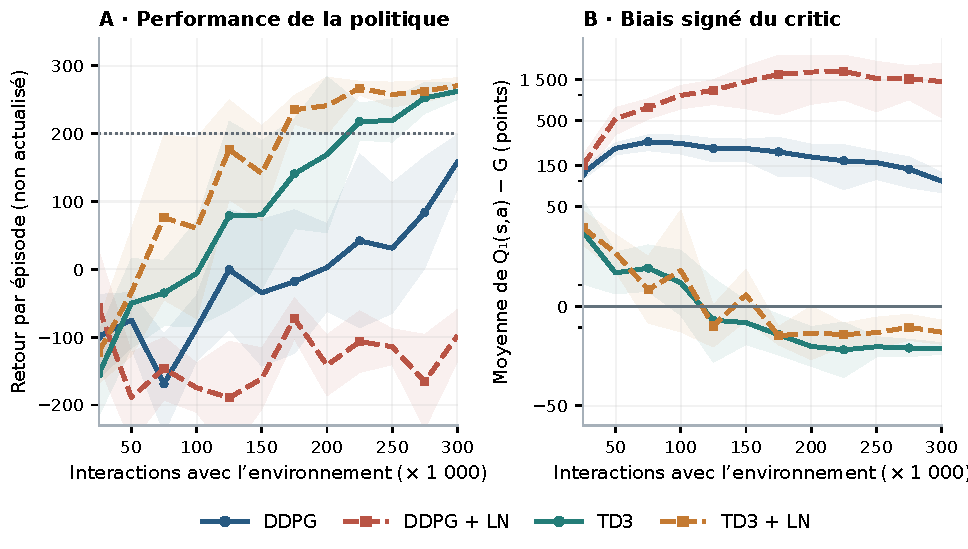
\includegraphics[width=.99\linewidth]{figure_evolution.pdf}
\caption{Évolution des quatre configurations, moyenne de cinq entraînements par configuration ; bandes : \emph{écart-type entre graines} (et non intervalle de confiance). À gauche, la performance est le retour épisodique \emph{non actualisé} ; à droite, le biais signé compare le critic au retour Monte-Carlo \emph{actualisé}. La ligne pointillée à 200 sert de repère ; l'axe des biais est symétrique-logarithmique.}
\label{fig:evolution}
\end{figure}
\vspace{-2pt}
\begin{table}[H]
\centering\small
\begin{tabular}{@{}lrrr@{}}
\toprule
\textbf{Configuration} & \textbf{Retour} & \textbf{Biais $Q_1-G$} & \textbf{Erreur $|Q_1-G|$} \\
\midrule
DDPG & $91 \pm 49$ & $+133 \pm 39$ & $133 \pm 39$ \\
DDPG + LN & $-126 \pm 29$ & $+1\,499 \pm 810$ & $1\,499 \pm 810$ \\
TD3 & $245 \pm 18$ & $-20 \pm 3$ & $25 \pm 5$ \\
TD3 + LN & $264 \pm 9$ & $-12 \pm 5$ & $19 \pm 4$ \\
\bottomrule
\end{tabular}
\caption{Valeurs finales : moyenne des checkpoints 250k, 275k et 300k, puis moyenne $\pm$ écart-type entre cinq graines. Le biais est signé ; la dernière colonne mesure $\E|Q_1-G|$ et inclut la variabilité des retours Monte-Carlo.}
\label{tab:resultats}
\end{table}
\vspace{-2pt}
\subsection{DDPG surestime ; TD3 présente un léger biais négatif}
Sans LN, DDPG garde en fin d'entraînement un biais positif de $+133\pm39$ points, tandis que TD3 aboutit à $-20\pm3$. Les cinq biais de TD3 sont tous inférieurs aux cinq biais de DDPG (séparation complète des groupes). La comparaison avec l'erreur absolue est instructive : pour DDPG, biais et erreur absolue sont presque égaux ($133$), ce qui traduit une surestimation très largement unidirectionnelle ; pour TD3, l'erreur absolue ($25$) est un peu supérieure à la sous-estimation moyenne ($20$), ce qui indique des écarts de signes différents selon les situations.

L'écart se retrouve dans le contrôle : le retour final moyen atteint $245$ avec TD3, contre $91$ avec DDPG. Le seuil indicatif de 200 points est franchi par TD3 dans ces évaluations, mais cela ne constitue pas, à lui seul, une certification formelle de résolution de l'environnement. DDPG progresse encore à la fin des 300\,000 interactions : nous comparons les méthodes à \emph{budget identique}, sans conclure sur leur comportement à convergence.

\subsection{LayerNorm amplifie la surestimation sous DDPG}
Avec LN, DDPG présente un biais final de $+1\,499$ points pour un retour de $-126$. L'échelle de l'erreur est remarquable : comme $\E[Q_1]=\E[Q_1-G]+\E[G]\geq\E[Q_1-G]-\E|G|$, et que $\E|G|\simeq49{,}5$ sur ces trajectoires, sa prédiction moyenne dépasse $1\,449$ points. Ce contraste avec les retours Monte-Carlo associés atteste une \emph{forte dérive des prédictions}, sans démontrer une divergence asymptotique.

Avec TD3, la LN rapproche le biais de zéro ($-12$ contre $-20$) et s'accompagne d'un retour moyen légèrement supérieur ($264$ contre $245$). Ce gain de performance reste incertain avec cinq entraînements par groupe.

\clearpage
\section{Analyse : contrastes et mécanismes}
\subsection{LayerNorm : une interaction qui dépend de l'algorithme}
Pour juger si les écarts dépassent les fluctuations entre entraînements, nous utilisons un \emph{test de permutation}. Si deux configurations avaient la même distribution de résultats, leurs dix observations (cinq chacune) pourraient échanger leurs étiquettes. Parmi les $\binom{10}{5}=252$ répartitions possibles, la \emph{valeur $p$} est la proportion donnant un écart de moyennes au moins aussi grand en valeur absolue que celui observé.
\begin{table}[H]
\centering\small
\begin{tabular}{@{}llrr@{}}
\toprule
\textbf{Comparaison (avant $\to$ après)} & \textbf{Mesure} & \textbf{Différence} & $\boldsymbol p$ \\
\midrule
DDPG $\to$ TD3 & Retour & $+154$ & $0{,}008$ \\
 & Biais & $-152$ & $0{,}008$ \\
DDPG $\to$ DDPG+LN & Retour & $-217$ & $0{,}008$ \\
 & Biais & $+1\,366$ & $0{,}008$ \\
TD3 $\to$ TD3+LN & Retour & $+19$ & $0{,}071$ \\
 & Biais & $+8$ & $0{,}024$ \\
\bottomrule
\end{tabular}

\caption{Écarts entre configurations : différence de moyennes = après $-$ avant. Chaque mesure (retour ou biais) possède son propre test bilatéral.}
\label{tab:contrastes}
\end{table}

Pour TD3 contre DDPG et pour l'ajout de LN à DDPG, $p=0{,}008$ sur le retour comme sur le biais : les groupes de cinq entraînements sont entièrement séparés. Dans TD3, LN réduit la sous-estimation ($+8$, $p=0{,}024$), mais le gain de retour ($+19$, $p=0{,}071$) reste incertain. Avec cinq graines et plusieurs tests, ces effets plus modestes demandent confirmation.

\begin{figure}[H]
\centering
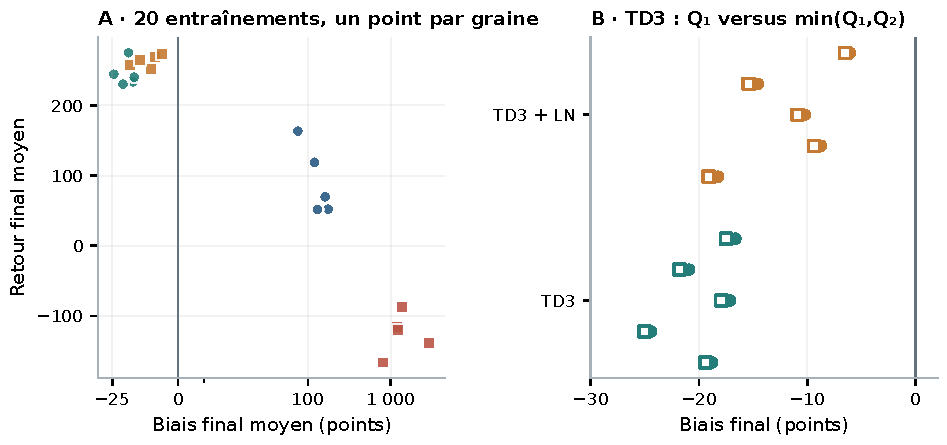
\includegraphics[width=.98\linewidth]{figure_details.pdf}
\caption{\textbf{A :} chaque point représente un entraînement indépendant (biais et retour final) ; couleurs et symboles de la figure~\ref{fig:evolution}. \textbf{B :} pour chaque graine TD3, un segment horizontal relie le biais de $Q_1$ (cercle plein) à celui de $\min(Q_1,Q_2)$ (carré creux) ; les deux symboles d'un même segment proviennent du \emph{même entraînement}.}
\label{fig:details}
\end{figure}

\subsection{TD3 : le minimum agit sur la cible, pas seulement sur la prédiction finale}
TD3 utilise $\min(Q_1,Q_2)$ pour construire les \emph{cibles de Bellman}. Or, sur les états effectivement évalués en fin d'entraînement, le biais de ce minimum est presque identique à celui de $Q_1$ ($-20{,}3$ contre $-19{,}6$ pour TD3 sans LN). Cela ne rend pas le mécanisme inutile : la cible agit au cours de toutes les mises à jour, alors que la figure compare des prédictions finales. La sous-estimation de TD3 ne peut donc pas être attribuée à un simple écart instantané entre ses deux critics.

\subsection{LayerNorm : activations bornées, valeurs non contrôlées}
La LN stabilise l'échelle des activations, mais ne borne pas uniformément les sorties du critic pendant l'entraînement. À paramètres fixés, en notant $\varphi$ les activations après la dernière LN et ReLU, $g,\beta$ ses paramètres affines, et $w,b$ les paramètres de sortie, on a
\begin{equation*}
\|\varphi\|_2\le\sqrt d\,\|g\|_\infty+\|\beta\|_2,\qquad
|Q|\le\|w\|_2\,\|\varphi\|_2+|b|.
\end{equation*}
Or $g,\beta,w,b$ sont eux-mêmes appris : ces bornes à paramètres fixés n'empêchent pas des prédictions croissantes lorsque les cibles de Bellman sont surestimées. Ce constat explique pourquoi la normalisation, à elle seule, ne garantit pas la calibration du critic.

\setstretch{0.97}
\setlength{\parskip}{1.0pt}
\titlespacing*{\subsection}{0pt}{3.5pt}{1pt}
\Needspace{16\baselineskip}
\subsection{Ablation DDPG : LN dans l'actor ou le critic}
Pour distinguer les deux emplacements, dix entraînements supplémentaires de DDPG utilisent LN dans un seul réseau (cinq par variante).
\begin{table}[H]
\centering\footnotesize
\begin{tabular}{@{}lrr@{}}
\toprule
\textbf{DDPG} & \textbf{Retour} & \textbf{Biais $Q_1-G$} \\
\midrule
Sans LN & $91 \pm 49$ & $+133 \pm 39$ \\
LN actor seul & $-82 \pm 64$ & $+352 \pm 123$ \\
LN critic seul & $-122 \pm 32$ & $+837 \pm 268$ \\
LN actor + critic & $-126 \pm 29$ & $+1\,499 \pm 810$ \\
\bottomrule
\end{tabular}
\caption{DDPG : moyenne $\pm$ écart-type sur cinq graines, mêmes checkpoints finaux que le tableau~\ref{tab:resultats}.}
\end{table}
\vspace{-5pt}
Sans LN, le biais vaut $+133$ ; il atteint $+352$ avec LN dans l'actor seul et $+837$ dans le critic seul ($p=0{,}008$ dans les deux cas, relativement à DDPG sans LN). L'effet est plus fort côté critic ($+485$ par rapport à l'actor seul, $p=0{,}008$). Normaliser les deux réseaux accroît encore le biais ($+1\,499$, $p=0{,}048$ par rapport au critic seul). Le retour chute dès qu'un seul réseau est normalisé ($-82$ et $-122$ contre $+91$ sans LN, $p=0{,}008$ dans les deux cas), mais reste voisin de $-126$ lorsque les deux le sont. Ainsi, des biais très différents s'accompagnent de retours pareillement dégradés.

\begingroup
\setstretch{0.97}
\setlength{\parskip}{1.0pt}
\titlespacing*{\subsection}{0pt}{3.5pt}{1pt}
\section{Discussion : mécanisme plausible et limites}
\subsection{Une rétroaction entre les deux réseaux}
DDPG ajuste son critic à des cibles de Bellman qui dépendent elles-mêmes de prédictions apprises. L'actor augmente ensuite la valeur prédite de ses actions : si celle-ci est excessivement optimiste, les décisions peuvent exploiter cette erreur et l'entretenir. TD3 introduit plusieurs mécanismes destinés à limiter cette rétroaction, ce qui est cohérent avec nos résultats, sans en identifier séparément les contributions.

\begin{center}

\begin{tikzpicture}[>=Latex, every node/.style={font=\footnotesize\sffamily, align=center}]
\node[draw=rulegray,fill=panelbg,rounded corners=2pt,minimum height=7mm,text width=39mm] (a) at (2.2,0) {Cible de Bellman\\surestimée};
\node[draw=rulegray,fill=panelbg,rounded corners=2pt,minimum height=7mm,text width=39mm] (b) at (8.15,0) {Critic ajusté\\vers cette cible};
\node[draw=rulegray,fill=panelbg,rounded corners=2pt,minimum height=7mm,text width=39mm] (c) at (14.1,0) {Actor attiré vers\\les actions surévaluées};
\draw[->,line width=.7pt,color=accent] (a)--(b);
\draw[->,line width=.7pt,color=accent] (b)--(c);
\draw[->,line width=.7pt,color=accent] (c.south)--++(0,-.25) -| (a.south);
\end{tikzpicture}
\end{center}
\vspace{-4pt}
\noindent{\footnotesize\color{muted}Mécanisme explicatif, non démontré causalement par cette comparaison.}

\subsection{Précision des mesures et portée des résultats}
\noindent\textbf{Précision des mesures.} Le retour Monte-Carlo $G_t$ est une réalisation aléatoire de la valeur que le critic cherche à estimer. La moyenne sur vingt épisodes réduit cette variabilité sans l'éliminer. De plus, un biais signé faible ne garantit pas un critic précis : des surestimations et des sous-estimations peuvent se compenser, d'où l'intérêt de mesurer également l'erreur absolue (tableau~\ref{tab:resultats}).

\noindent\textbf{Portée des comparaisons.} Les tests statistiques portent sur les entraînements indépendants, et non sur les états-actions observés au cours d'une même trajectoire. Avec cinq graines par configuration, les différences les plus marquées sont bien mises en évidence, mais les effets plus modestes restent incertains. Enfin, nos conclusions concernent LunarLander-v3 après 300\,000 interactions ; DDPG progressant encore à ce stade, elles ne préjugent pas de son comportement après un entraînement plus long.

\subsection{Ce que l'expérience ne permet pas d'attribuer}
La comparaison montre à la fois de meilleures performances et un critic moins surestimatif sous TD3. Cependant, TD3 modifie conjointement le minimum des critics, le lissage des actions cibles et la fréquence de mise à jour de l'actor. \textbf{Nous ne pouvons donc pas attribuer le gain de performance à la seule réduction du biais.} L'ablation précise l'effet du placement de LN dans DDPG, mais ne permet pas d'établir le mécanisme reliant ce placement aux erreurs de valeur.

\subsection{Expériences complémentaires ciblées}
\textbf{(i)} Reproduire l'ablation LN dans TD3. \textbf{(ii)} Retirer séparément les trois modifications de TD3 pour mesurer leurs contributions. \textbf{(iii)} Augmenter le nombre de graines et prolonger les entraînements pour évaluer la stabilité des contrastes. Ces expériences ne figurent pas dans les résultats présentés ; l'ensemble des données utilisées ici est disponible dans \texttt{results/*/evaluations.csv}.

\vspace{4pt}
\noindent{\sffamily\bfseries\color{navy} Conclusion.}\quad
Sur cette tâche et à budget égal, TD3 associe un critic nettement moins surestimatif à une politique plus performante. La LN aggrave la surestimation de DDPG, y compris lorsqu'elle est limitée à l'actor ou au critic, mais pas celle de TD3. Elle ne corrige donc pas, à elle seule, les erreurs d'estimation des valeurs.

\vspace{5pt}
\noindent{\color{rulegray}\rule{\linewidth}{.55pt}}
\vspace{-5pt}
{\footnotesize
\begin{english}\renewcommand{\refname}{Références}\begin{thebibliography}{9}\setlength{\itemsep}{0pt}\setlength{\parsep}{0pt}
\bibitem{ba2016} J. L. Ba, J. R. Kiros, G. E. Hinton. \emph{Layer Normalization}. arXiv:1607.06450, 2016.
\bibitem{fujimoto2018} S. Fujimoto, H. van Hoof, D. Meger. \emph{Addressing Function Approximation Error in Actor-Critic Methods}. ICML, 2018.
\bibitem{lillicrap2016} T. Lillicrap et al. \emph{Continuous Control with Deep Reinforcement Learning}. ICLR, 2016.
\bibitem{pardo2018} F. Pardo et al. \emph{Time Limits in Reinforcement Learning}. ICML, 2018.
\bibitem{towers2024} M. Towers et al. \emph{Gymnasium: A Standard Interface for Reinforcement Learning Environments}. arXiv:2407.17032, 2024.
\bibitem{vanhasselt2010} H. van Hasselt. \emph{Double Q-learning}. NeurIPS, 2010.
\end{thebibliography}\end{english}
}
\endgroup
\end{document}
